%==============================================================
% PE5 - Práctica Experimental Unidad V
% Integración, Métricas y Defensa del Proyecto Integrador de IR
% Sistema: CarniCore
% Universidad Técnica Estatal de Quevedo (UTEQ)
% Asignatura: Ingeniería de Requerimientos [20303] - ISR-401
% Versión: 4.0 - Agosto 2026

%==============================================================

\documentclass[11pt,a4paper]{article}

%--- Paquetes ---
\usepackage[utf8]{inputenc}
\usepackage[T1]{fontenc}
\usepackage[spanish,es-tabla]{babel}
\usepackage{geometry}
\geometry{top=2.5cm, bottom=2.5cm, left=2.5cm, right=2.5cm, headheight=14pt}
\usepackage{longtable}
\usepackage{booktabs}
\usepackage{array}
\usepackage{colortbl}
\usepackage{xcolor}
\usepackage{graphicx}
\usepackage{hyperref}
\usepackage{enumitem}
\usepackage{titlesec}
\usepackage{fancyhdr}
\usepackage{tabularx}
\usepackage{multirow}
\usepackage{amsmath}
\usepackage{amssymb}
\usepackage{float}
\usepackage{setspace}
\usepackage{caption}
\usepackage{subcaption}
\usepackage{tocloft}
\usepackage{url}
\usepackage{cite}

%--- Colores ---
\definecolor{uteqblue}{RGB}{0,70,130}
\definecolor{lightgray}{RGB}{240,240,240}
\definecolor{trelloblue}{RGB}{0,82,204}

%--- Rutas de figuras ---
\graphicspath{{figuras/}}

%--- Hipervínculos ---
\hypersetup{
  colorlinks=true,
  linkcolor=uteqblue,
  citecolor=uteqblue,
  urlcolor=blue,
  pdftitle={PE5 - Informe Final CarniCore},
  pdfauthor={Equipo CarniCore - UTEQ ISR-401}
}

%--- Encabezado y pie de página ---
\pagestyle{fancy}
\fancyhf{}
\fancyhead[L]{\small UTEQ -- Ingeniería de Requerimientos (ISR-401/20303)}
\fancyhead[R]{\small PE5 -- CarniCore -- Informe Final}
\fancyfoot[C]{\thepage}
\renewcommand{\headrulewidth}{0.4pt}

%--- Numeración de figuras y tablas ---
\counterwithin{figure}{section}
\counterwithin{table}{section}

%==============================================================
\begin{document}
%==============================================================

%--- PORTADA ---
\begin{titlepage}
  \centering
  \vspace*{0.3cm}

  {\large \textbf{UNIVERSIDAD TÉCNICA ESTATAL DE QUEVEDO}}\\[0.2cm]
  {\large \textbf{FACULTAD DE CIENCIAS DE LA COMPUTACIÓN Y DISEÑO DIGITAL}}\\[0.2cm]
  {\large \textbf{CARRERA DE INGENIERÍA DE SOFTWARE (REDISEÑO)}}\\[0.4cm]

  
\includegraphics[width=4cm]{figuras/logo.png}\\[0.1cm]

  \rule{\textwidth}{1pt}\\[0.1cm]
  {\LARGE \textbf{PRÁCTICA EXPERIMENTAL UNIDAD V (PE5)}}\\[0.1cm]
  {\Large \textbf{Integración, Métricas y Defensa del Proyecto Integrador\\de Ingeniería de Requisitos}}\\[0.1cm]
  \rule{\textwidth}{1pt}\\[0.2cm]

  {\large \textbf{PROYECTO:}}\\[0.15cm]
  {\Large \textbf{CarniCore}}\\[0.15cm]
  {\normalsize Sistema de Trazabilidad, Pesaje Inteligente e Inventario para\\
  Distribuidora de Cárnicos Pucayacu -- La Maná, Cotopaxi}\\[0.4cm]

  {\large \textbf{INTEGRANTES:}}\\[0.3cm]
  \begin{tabular}{|p{7.5cm}|p{4cm}|}
    \hline
    \rowcolor{uteqblue!15}
    \textbf{Nombre} & \textbf{Cédula} \\
    \hline
    CASTRO BAJAÑA ARIEL OMAR      & 2350262305 \\[0.35cm]
    \hline
    CRESPO ESPINOZA KLEBER OBED      & 1315380244 \\[0.35cm]
    \hline
    GAMARRA ARAUJO EDHU XAVIER       & 1208370633 \\[0.35cm]
    \hline
    PÉREZ RUIZ CARLOS ANDRÉS       & 0955713136 \\[0.35cm]
    \hline
    QUINTERO GENDE ERICK JAHIR       & 1250575527 \\[0.35cm]
    \hline
  \end{tabular}\\[0.4cm]

  {\large \textbf{ASIGNATURA:}} Ingeniería de Requerimientos [20303] -- ISR-401\\[0.30cm]
  {\large \textbf{CURSO:}} 4to ``A'' Software\\[0.30cm]
  {\large \textbf{DOCENTE:}} PhD. Guerrero Ulloa Gleiston Cicerón\\[0.30cm]
  {\large \textbf{PERIODO:}} 2026-2027 PPA\\[0.30cm]
  {\large \textbf{FECHA:}} Agosto 21 del 2026\\[0.30cm]
    {\large \textbf{REVISION:}} Último commit aceptado hasta el Viernes 21 de Agosto 23:55\\[0.30cm]


  % ===== REPOSITORIO EN UNA LÍNEA SOLITARIA (CRITERIO DE PISO G1) =====
  {\large \textbf{REPOSITORIO:}}

  \url{https://github.com/EdhuXav/PE5_ISR401_GRUPO_CCGaPQ}

\end{titlepage}

%--- RESUMEN BILINGÜE ---
\newpage
\section*{Resumen}
\addcontentsline{toc}{section}{Resumen}

El presente informe corresponde a la Práctica Experimental Unidad V (PE5) de Ingeniería de Requerimientos (ISR-401) y consolida el cierre del Proyecto Integrador CarniCore, sistema de trazabilidad, pesaje inteligente e inventario para una distribuidora de productos cárnicos de Pucayacu, La Maná, Cotopaxi. La auditoría de calidad se aplicó sobre los 40 requisitos base del ERS/SRS (25 RF y 15 RNF), mientras que los 18 requisitos de inteligencia artificial se controlan como extensión específica de la PE5. En la versión v4.0: M1a alcanzó 97,5\% de completitud de atributos; M2 obtuvo 1,0000 de consistencia; M3 alcanzó 97,5\% de verificabilidad; M4 registró 96,0\% de trazabilidad hacia adelante y 100\% hacia atrás; M5 obtuvo 2,71 requisitos afectados en promedio; y M6 cerró en 0,00 defectos residuales por requisito. La matriz consolidada contempla 60 filas: 42 requisitos base (27 RF + 15 RNF) y 18 de IA. Se especificaron dos componentes de inteligencia artificial plausibles para el dominio: un predictor de demanda por tipo de corte (IA-01) y un detector de anomalías de cadena de frío (IA-02), cada uno con requisitos de rendimiento, equidad, explicabilidad, plan de fallback y monitoreo. El documento integra además la validación del ERS derivada de la inspección Fagan de la PE4, la gestión de cambios mediante CCB, la retrospectiva de equipo en formato Start-Stop-Continue y cinco conclusiones integradoras vinculadas a las unidades de la asignatura. La gestión del proyecto se realizó en Trello (\url{https://trello.com/b/CCGaPQ}).

\textbf{Palabras clave:} ingeniería de requisitos, trazabilidad de software, métricas de calidad, ISO/IEC 25010:2023, inteligencia artificial, trazabilidad cárnica, ERS/SRS, inspección Fagan, CarniCore.

\vspace{1cm}

\section*{Abstract}
\addcontentsline{toc}{section}{Abstract}

This report corresponds to Experimental Practice Unit V (PE5) of the Requirements Engineering course (ISR-401) and consolidates the closure of the CarniCore Integrative Project, a traceability, intelligent weighing and inventory system for a meat products distributor in Pucayacu, La Maná, Cotopaxi. The quality audit was applied to the 40 base SRS requirements (25 functional and 15 non-functional), while the 18 artificial intelligence requirements are controlled as a PE5-specific extension. In version v4.0: M1a reached 97.5\% attribute completeness; M2 obtained 1.0000 consistency; M3 reached 97.5\% verifiability; M4 achieved 96.0\% forward traceability and 100\% backward traceability; M5 yielded an average of 2.71 affected requirements; and M6 closed at 0.00 residual defects per requirement. The consolidated traceability matrix contains 60 rows: 42 base requirements (27 functional and 15 non-functional) and 18 AI requirements. Two AI components plausible for the domain were specified: a demand predictor by cut type (IA-01) and a cold-chain anomaly detector (IA-02), each with performance, fairness, explainability, fallback, and monitoring requirements. The report also integrates SRS validation derived from the Fagan inspection of PE4, change management through the CCB, the team retrospective in Start-Stop-Continue format, and five integrating conclusions linked to the five course units. Project management was performed using Trello (\url{https://trello.com/b/CCGaPQ}).

\textbf{Keywords:} requirements engineering, software traceability, quality metrics, ISO/IEC 25010:2023, artificial intelligence, meat traceability, SRS, Fagan inspection, CarniCore.

%--- ÍNDICES ---
\newpage
\tableofcontents
\newpage
\listoftables
\newpage
\listoffigures
\newpage

%--- HISTORIAL DE VERSIONES ---
\section*{Historial de Versiones del Documento}
\addcontentsline{toc}{section}{Historial de Versiones}
\begin{longtable}{|p{1.5cm}|p{2.5cm}|p{3.5cm}|p{7cm}|}
\hline
\textbf{Versión} & \textbf{Fecha} & \textbf{Autor(es)} & \textbf{Descripción} \\
\hline
1.0 & 31/05/2026 & Equipo CarniCore & PE1 -- Planificación del proyecto de IR y descripción general preliminar. \\
\hline
1.5 & 15/06/2026 & Equipo CarniCore & Correcciones PE1: alcance delimitado, exclusión de facturación SRI. \\
\hline
2.0 & 12/07/2026 & Equipo CarniCore & PE2 -- Interfaces externas, 15 RF, 6 RNF, modelado UML parcial. \\
\hline
3.0 & 02/08/2026 & Equipo CarniCore & PE3/PE4 -- ERS completo (25 RF, 15 RNF), modelos UML completos, inspección Fagan (17 defectos), CCB (RFC-01 a RFC-03), trazabilidad extendida, línea base v1.1 etiquetada. \\
\hline
4.0 & 21/08/2026 & Equipo CarniCore & PE5 -- Integración final, auditoría de calidad con seis métricas ISO/IEC 25010:2023, trazabilidad end-to-end consolidada (60 filas: 42 base + 18 IA), incorporación de RF-26 y RF-27, requisitos de IA (IA-01 e IA-02) y retrospectiva de cierre. \\
\hline
\caption{Historial de versiones del documento PE5 -- CarniCore}
\label{tab:historial}
\end{longtable}

%==============================================================
\section{Introducción}
%==============================================================

\subsection{Problema y Contexto}

La distribuidora de productos cárnicos Pucayacu, ubicada en La Maná, provincia de Cotopaxi, Ecuador, operaba en 2026 con un sistema de gestión completamente manual: los registros de ingreso de animales, pesaje, inventario en cámaras frigoríficas, bajas por vencimiento y reportes de ventas se realizaban en cuadernos físicos y hojas de cálculo en Excel sin ningún mecanismo de trazabilidad integrado. Esta situación generaba tres tipos de riesgo verificables: (i) pérdidas económicas por vencimiento de producto no detectado a tiempo, (ii) riesgo regulatorio ante Agrocalidad al no poder acreditar la cadena de trazabilidad exigida desde la granja de origen hasta la venta, y (iii) diferencias de inventario no explicadas entre el registro manual y el conteo físico semanal \cite{pohl2025}.

El sistema CarniCore fue diseñado para resolver estos problemas mediante la digitalización y trazabilidad de los procesos operativos críticos, incluyendo la gestión de proveedores y guías de origen, el pesaje inteligente con cálculo automático de costos, el control de inventario en cámaras frigoríficas, las alertas de vida útil, y la generación de reportes gerenciales exportables. La elicitación de requisitos se realizó mediante entrevistas semiestructuradas con la propietaria, el administrador general, el encargado de bodega y el carnicero principal, complementadas con observación directa en la planta de La Maná.

\subsection{Objetivos del Informe Final}

Este informe final integra los resultados de las cinco unidades de la asignatura Ingeniería de Requerimientos (ISR-401) con los siguientes objetivos específicos:

\begin{enumerate}
  \item Auditar la calidad del ERS/SRS final con seis métricas derivadas de ISO/IEC 25010:2023 \cite{iso25010}, mostrando la aritmética completa y el par antes/después de cada corrección.
  \item Verificar y cerrar la trazabilidad end-to-end desde las fuentes de stakeholders hasta los casos de prueba conceptuales, eliminando requisitos huérfanos y cadenas rotas.
  \item Especificar los requisitos de dos componentes de inteligencia artificial plausibles para CarniCore, con sus dimensiones funcionales, de rendimiento, equidad y explicabilidad.
  \item Presentar la versión final integrada del ERS/SRS v4.0, coherente con ISO/IEC/IEEE 29148:2018 \cite{iso29148}.
  \item Documentar la retrospectiva de equipo y formular cinco conclusiones integradoras específicas del proyecto.
\end{enumerate}

\subsection{Estructura del Documento}

El documento se organiza en diez secciones de contenido, conforme a la estructura exigida en la Guía PE5: Sección~\ref{sec:metodologia} presenta la metodología de IR seguida en las cinco unidades; Sección~\ref{sec:ers} describe la estructura y requisitos clave del ERS/SRS final; Sección~\ref{sec:uml} incluye los modelos UML con lectura interpretativa; Sección~\ref{sec:validacion} documenta la validación, inspección y correcciones derivadas de la PE4; Sección~\ref{sec:trazabilidad} presenta la gestión, línea base y matriz de trazabilidad final; Sección~\ref{sec:ia} especifica los requisitos de los componentes de IA; Sección~\ref{sec:metricas} contiene la auditoría de calidad con la aritmética de cada métrica; Sección~\ref{sec:retrospectiva} documenta la retrospectiva Start-Stop-Continue; y Sección~\ref{sec:conclusiones} formula las conclusiones integradoras.

Los artefactos de esta práctica se organizan en el repositorio \url{https://github.com/EdhuXav/PE5_ISR401_GRUPO_CCGaPQ} de la siguiente manera: el informe LaTeX (\texttt{main.tex}, \texttt{referencias.bib} y carpeta \texttt{figuras/}) se ubica en \texttt{informe/}; la hoja de métricas de IA en \texttt{metricas\_IA/}; las diapositivas de defensa y banco de preguntas en \texttt{defensa/}; y la matriz de trazabilidad final en \texttt{trazabilidad/}.

%==============================================================
\section{Metodología de Ingeniería de Requisitos}
\label{sec:metodologia}
%==============================================================

\subsection{Marco Normativo Aplicado}

El proyecto CarniCore aplicó la metodología de ingeniería de requisitos conforme a ISO/IEC/IEEE 29148:2018 \cite{iso29148} como estándar rector de la especificación, y a ISO/IEC 25010:2023 \cite{iso25010} como modelo de calidad del producto documental. El encuadre de procesos de ciclo de vida siguió ISO/IEC/IEEE 15288:2023 para sistemas \cite{iso15288} y ISO/IEC/IEEE 12207:2017 para software \cite{iso12207}. Los fundamentos conceptuales se apoyaron en Pohl \cite{pohl2025} y en el SWEBOK v4.0 \cite{swebok2024}; la gestión del proyecto integrador siguió los principios del PMBOK 7.ª edición \cite{pmbok7}; y la terminología de cualificación se alineó con el temario IREB CPRE Foundation Level v3.3.0 \cite{ireb330}.

\subsection{Justificación del Enfoque Metodológico Seleccionado}

La elección de ISO/IEC/IEEE 29148:2018 \cite{iso29148} como estándar rector para la especificación no fue trivial: el equipo evaluó también el uso del marco ágil puro (solo historias de usuario y criterios de aceptación Gherkin sin documento SRS formal). Se optó por el enfoque híbrido ---documento SRS estructurado más backlog de Trello con historias Connextra+Gherkin--- por tres razones concretas del dominio de CarniCore:

\begin{enumerate}
  \item \textbf{Exigencia regulatoria:} Agrocalidad requiere evidencia documental de la cadena de trazabilidad. Un backlog de Trello sin artefacto SRS no proporciona la auditabilidad requerida.
  \item \textbf{Restricciones de diseño explícitas:} Las restricciones RD-1 a RD-4 (identificación dual, exclusión de facturación SRI, continuidad offline, motor relacional) son contratos con el cliente que deben ser inequívocamente documentables, con versiones etiquetadas y trazabilidad de cambios.
  \item \textbf{Contexto educativo:} La asignatura exige la aplicación de las cinco unidades de IR de forma progresiva, lo que hace del SRS el artefacto central de integración.
\end{enumerate}

\subsection{Gestión del Proyecto con Trello}

La gestión del proyecto integrador se realizó en Trello, herramienta declarada en el informe y utilizada de forma consistente en todas las prácticas. El tablero del proyecto se encuentra en:

\begin{center}
  \url{https://trello.com/invite/b/6a88f70b4989d755a6cfe8f9/ATTI4653fd9584f182a3522e85a8f8fd1c3c5946D5E6/carnicore-pe5}
\end{center}

% -------------------------------------------------------
% CAPTURA TRELLO 1: Vista general del tablero
% -------------------------------------------------------
% Instrucción: Guarda la captura como "figuras/trello_tablero_general.png"
% La imagen debe mostrar el tablero completo con todas las listas visibles.
% Tamaño recomendado: ancho completo, resolución mínima 1200 px.
\begin{figure}[H]
  \centering
  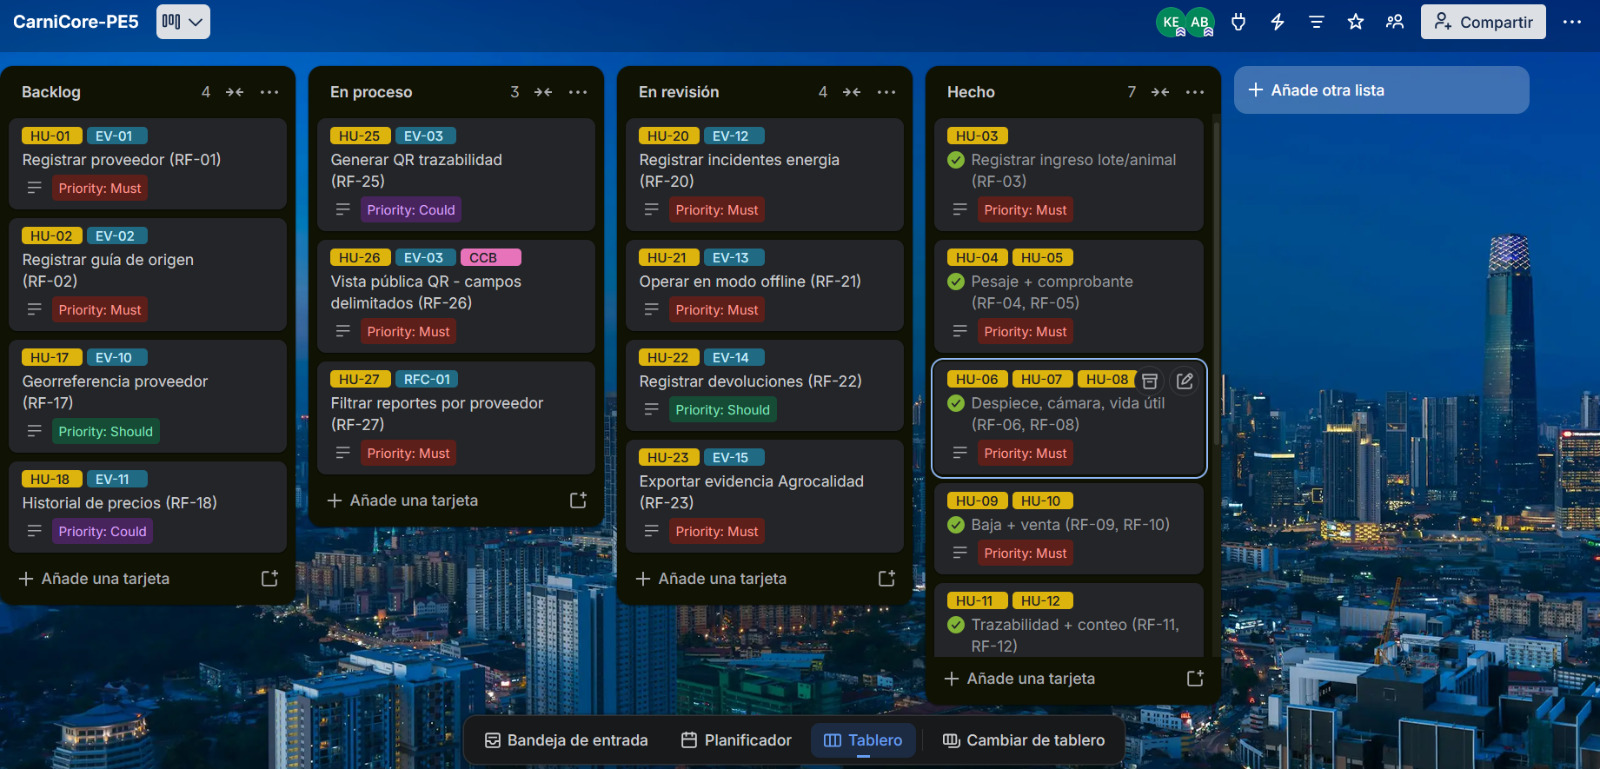
\includegraphics[width=0.85\linewidth]{figuras/trello_tablero_general.png}
  \caption{Tablero Trello del proyecto CarniCore - vista general}
  \label{fig:contexto}
\end{figure}

El tablero de Trello organiza el \textit{product backlog} en cinco épicas (EPIC-01 a EPIC-05) mapeadas a listas: ``Backlog'', ``Sprint activo'', ``En revisión'' y ``Hecho''. Cada tarjeta lleva etiquetas de prioridad MoSCoW, la fuente del requisito (EV-XX), el responsable del integrante y el criterio de aceptación en formato BDD. Esta estructura garantiza la sincronización entre el ERS y el backlog exigida por la Guía PE5 (Paso 2.d) \cite{hoy2023}.

\subsection{Proceso Seguido en las Cinco Unidades}

El proceso de IR del proyecto CarniCore siguió un enfoque iterativo con cinco fases sincronizadas con las unidades de la asignatura:

\begin{description}
  \item[PE1 -- Unidad I (Planificación y Elicitación):] Se identificaron los stakeholders mediante una matriz poder/interés, se realizó la primera ronda de entrevistas semiestructuradas con la propietaria y se estableció el plan del proyecto con cronograma de 17 semanas. Se obtuvieron las evidencias EV-01 a EV-09 que sustentan los RF-01 a RF-16.

  \item[PE2 -- Unidad II (Especificación):] Se documentaron 15 RF, 6 RNF, las interfaces externas con mockups de baja fidelidad (P1--P6) y el modelado UML parcial. Se estableció la primera versión de la matriz de trazabilidad parcial y se aplicó la priorización MoSCoW.

  \item[PE3 -- Unidad III (Modelado y Segunda Elicitación):] Se completó el ERS a 25 RF y 15 RNF con todos los atributos exigidos. Se realizó la segunda ronda de elicitación (semana 12), obteniendo las evidencias EV-10 a EV-15 que sustentaron los RF-17 a RF-25. Se elaboraron los 20 mockups de alta fidelidad (MU-01 a MU-20) y el modelado UML completo.

  \item[PE4 -- Unidad IV (Validación y Gestión):] Se ejecutó la inspección formal Fagan del ERS v1.0, detectando 17 defectos. Se tramitaron tres RFC ante el CCB simulado. Se estableció la línea base v1.1 con etiqueta Git. La trazabilidad se implementó en Trello con cinco épicas y 24 tarjetas de historia de usuario.

  \item[PE5 -- Unidad V (Integración, Métricas y Cierre):] Se realizó la auditoría de calidad con las seis métricas ISO/IEC 25010:2023, se verificó y cerró la trazabilidad end-to-end, se especificaron los requisitos de los dos componentes de IA y se consolidó la versión final v4.0 del ERS.
\end{description}

% -------------------------------------------------------
% CAPTURA TRELLO 2: Lista de historias de usuario (backlog)
% -------------------------------------------------------
% Instrucción: Guarda la captura como "figuras/trello_backlog.png"
% Debe mostrar las tarjetas HU-01 a HU-27 con etiquetas y asignados.
\begin{figure}[H]
  \centering
  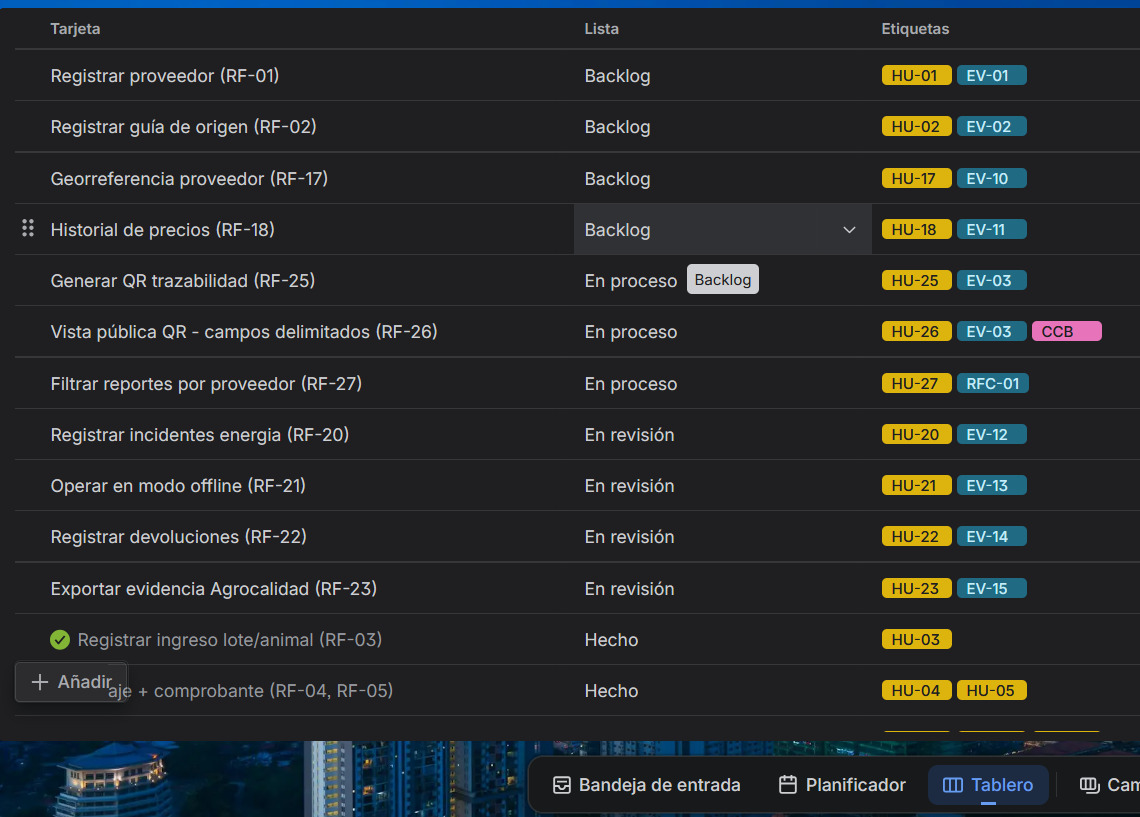
\includegraphics[width=0.85\linewidth]{figuras/trello_backlog.png}
  \caption{Backlog del proyecto en Trello -- historias de usuario HU-01 a HU-27}
  \label{fig:contexto}
\end{figure}


\subsection{Técnicas de Elicitación y Decisiones Metodológicas}

La técnica principal de elicitación fue la \textbf{entrevista semiestructurada}, seleccionada por su adecuación a un dominio con un único cliente experto (la propietaria) y una organización pequeña con conocimiento tácito no documentado. Se realizaron cinco entrevistas en dos rondas. La primera ronda (semanas 3--4) cubrió los procesos de proveedores, pesaje, inventario y reportes; la segunda ronda (semana 12) cubrió los procesos de gestión de incidentes de corte de energía, devoluciones, exportación para Agrocalidad y continuidad offline.

Como técnica complementaria se usó la \textbf{observación directa} en la planta de La Maná, que permitió identificar RF-20 (registro de incidentes de corte de energía) y RF-21 (modo offline) como requisitos no verbalizados espontáneamente por los usuarios pero evidentes en el entorno operativo. Se aplicó también un \textbf{cuestionario} a tres perfiles de usuario para validar cuantitativamente RNF-04 (usabilidad) y RNF-14 (recuperabilidad offline).

\subsection{Comparativa de Técnicas de Elicitación Evaluadas}

\begin{table}[H]
\centering
\begin{tabular}{|p{3cm}|p{3cm}|p{3cm}|p{4cm}|}
\hline
\textbf{Técnica} & \textbf{Ventajas} & \textbf{Limitaciones} & \textbf{Decisión} \\
\hline
Entrevista semiestructurada & Alta profundidad; permite seguir líneas inesperadas & Dependiente del entrevistador; sin comparabilidad directa & \textbf{Seleccionada} (técnica principal) \\
\hline
Cuestionario & Escalable; anónimo & Superficial; sin posibilidad de aclaración & Complementaria (validación RNF-04, RNF-14) \\
\hline
Observación directa & Detecta requisitos no verbalizados & Intrusiva; costosa en tiempo & \textbf{Seleccionada} (complementaria; descubrió RF-20 y RF-21) \\
\hline
Taller de requisitos & Alta participación; valida in-situ & Requiere disponibilidad simultánea de todos los stakeholders & Descartada (propietaria y bodega tienen horarios incompatibles) \\
\hline
\end{tabular}
\caption{Evaluación de técnicas de elicitación consideradas para CarniCore}
\label{tab:tecnicas}
\end{table}

\subsection{Registro de Evidencias de Elicitación}

\begin{longtable}{|p{1cm}|p{2cm}|p{2cm}|p{2.5cm}|p{3cm}|p{3cm}|}
\hline
\textbf{EV} & \textbf{Fecha} & \textbf{Técnica} & \textbf{Stakeholder} & \textbf{Contenido principal} & \textbf{RF sustentados} \\
\hline
EV-01 & Sem. 3 & Entrevista & Propietaria & Registro de proveedores y control de acceso al sistema & RF-01, RF-15 \\
EV-02 & Sem. 3 & Entrevista & Propietaria & Requerimiento de guía de origen para cada lote & RF-02 \\
EV-03 & Sem. 3 & Entrevista & Propietaria & Identificación individual de animales (arete) y por lote (aves) & RF-03, RF-11, RF-25 \\
EV-04 & Sem. 4 & Entrevista & Propietaria & Proceso de pesaje con cálculo de costo y emisión de comprobante & RF-04, RF-05 \\
EV-05 & Sem. 4 & Entrevista & Carnicero & Proceso de despiece y clasificación por tipo de corte & RF-06 \\
EV-06 & Sem. 4 & Entrevista & Propietaria & Gestión de cámaras frigoríficas y control de vida útil & RF-07, RF-08 \\
EV-07 & Sem. 4 & Entrevista & Propietaria & Proceso de baja de producto con causa y aprobación & RF-09 \\
EV-08 & Sem. 4 & Entrevista & Propietaria & Registro de ventas, reportes gerenciales y panel resumen & RF-10, RF-13, RF-14 \\
EV-09 & Sem. 4 & Observación & Bodega & Conteo físico semanal de inventario, búsqueda de productos & RF-12, RF-16, RF-24 \\
EV-10 & Sem. 12 & Entrevista & Admin. general & Necesidad de georreferenciación de proveedores para auditorías & RF-17 \\
EV-11 & Sem. 12 & Entrevista & Propietaria & Gestión de precios por temporada e historial de precios & RF-18, RF-19 \\
EV-12 & Sem. 12 & Entrevista & Propietaria & Registro de incidentes de corte de energía y pérdidas asociadas & RF-20 \\
EV-13 & Sem. 12 & Entrevista & Bodega & Operación sin internet: necesidad de modo offline & RF-21 \\
EV-14 & Sem. 12 & Entrevista & Bodega & Proceso de devoluciones y reingreso al inventario & RF-22 \\
EV-15 & Sem. 12 & Entrevista & Admin. general & Exportación de evidencia para inspecciones de Agrocalidad & RF-23 \\
\hline
\caption{Registro de evidencias de elicitación -- CarniCore (dos rondas)}
\label{tab:evidencias}
\end{longtable}

\subsection{Priorización de Requisitos: MoSCoW, Kano y WSJF}

El ERS v4.0 aplica una priorización combinada de tres modelos \cite{pmbok7}: de los 27 RF totales, 19 son Must (70,4\%), 6 son Should (22,2\%) y 2 son Could (7,4\%). Para los RF Must originales, el WSJF arrojó mayor prioridad a RF-08 (vida útil, WSJF = 4,2), RF-11 (trazabilidad, WSJF = 3,8) y RF-04 (pesaje, WSJF = 3,5). La Figura~\ref{fig:wsjf} ilustra la distribución del WSJF por RF Must.

\begin{figure}[H]
  \centering
  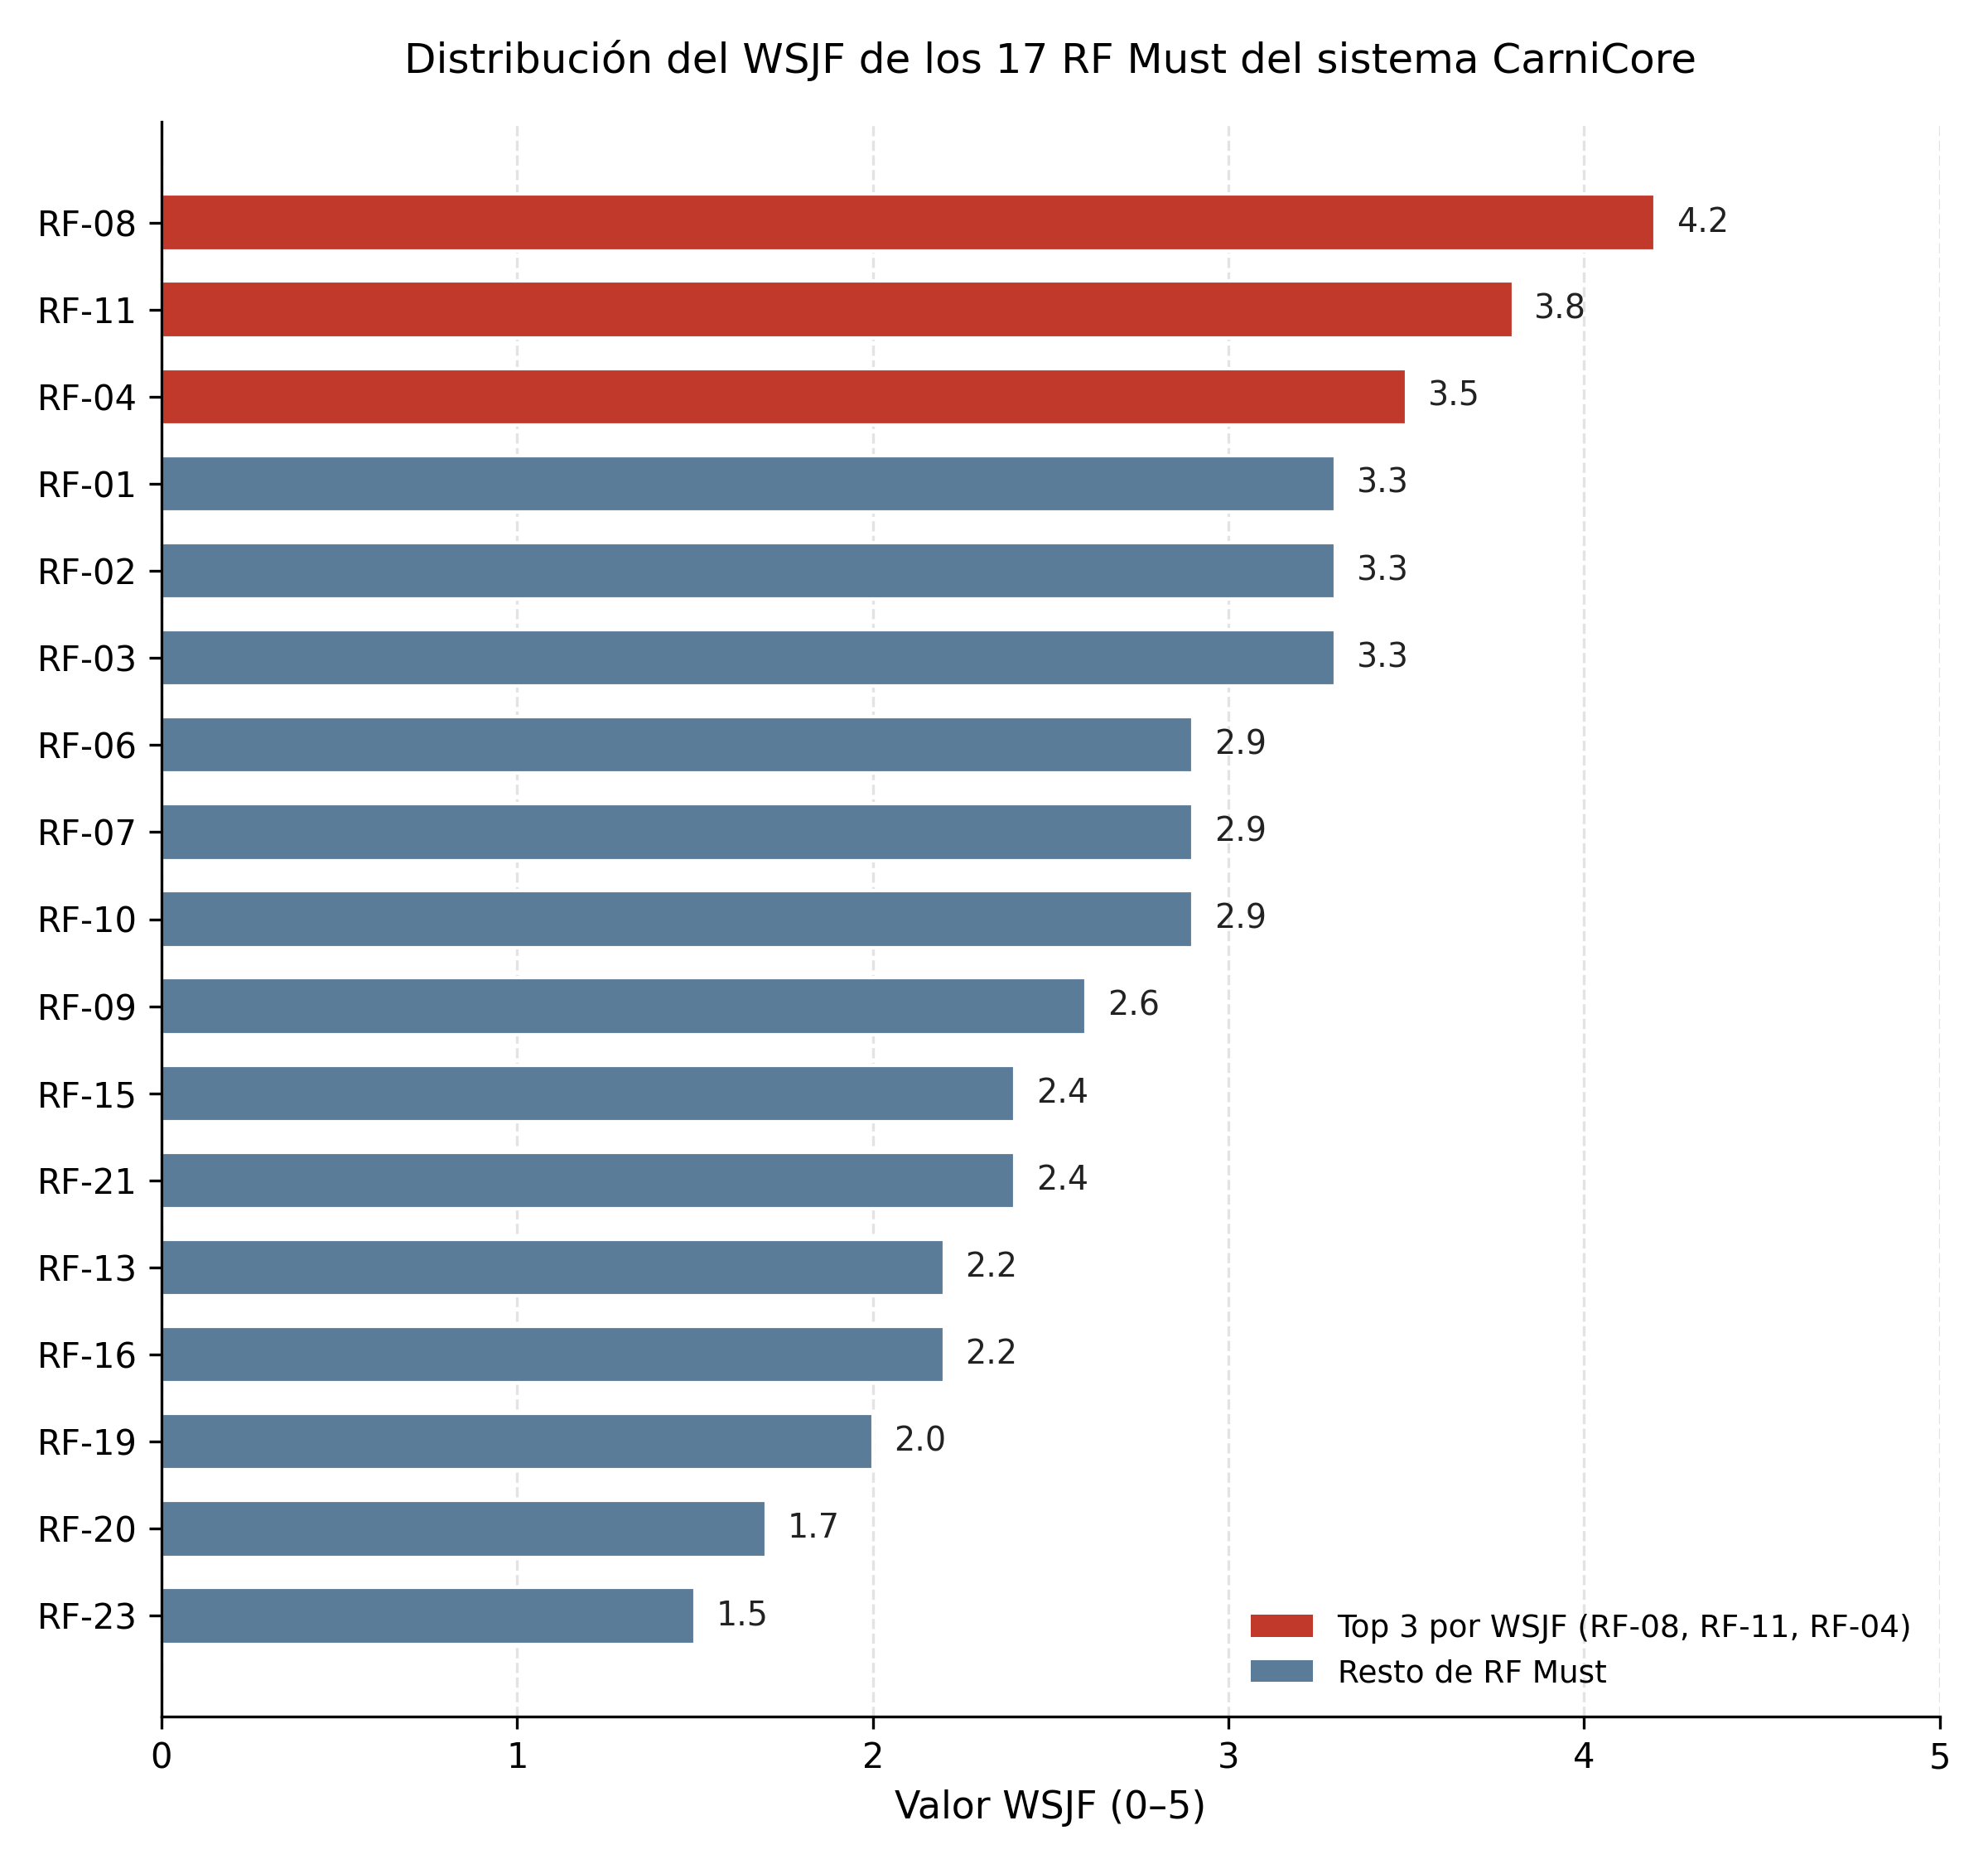
\includegraphics[width=0.9\linewidth]{figuras/WSJF_RF_Must.png}
  \caption{Distribución WSJF de los 17 RF Must del sistema CarniCore}
  \label{fig:wsjf}
\end{figure}

%==============================================================


%--- REFERENCIAS ---
\newpage
\bibliographystyle{IEEEtran}
\bibliography{referencias}



\end{document}
